\documentclass[a4paper]{report}
\usepackage{setspace}

\pagestyle{plain}
\usepackage{amssymb}
\usepackage{graphicx}
\usepackage{color}
\usepackage{amsfonts}
\usepackage{latexsym}
\usepackage{amsmath}
\usepackage[toc,page]{appendix}
\setcounter{tocdepth}{1}
\usepackage{pdfpages}
\usepackage{todonotes}
\usepackage{hyperref}
\hypersetup{
    colorlinks,
    citecolor=black,
    filecolor=black,
    linkcolor=black,
    urlcolor=black
}

\usepackage[authoryear]{natbib}
\usepackage{algorithm}
\usepackage{algpseudocode}

% \usepackage{caption}
\usepackage{subcaption}
\usepackage{float}
\usepackage{lipsum}
\usepackage[a4paper, margin = 3cm, bottom = 2.5cm]{geometry}

\newtheorem{theorem}{THEOREM}
\newtheorem{lemma}[theorem]{LEMMA}
\newtheorem{corollary}[theorem]{COROLLARY}
\newtheorem{proposition}[theorem]{PROPOSITION}
\newtheorem{remark}[theorem]{REMARK}
\newtheorem{definition}[theorem]{DEFINITION}
\newtheorem{fact}[theorem]{FACT}

\newcommand{\nats}{\mbox{\( \mathbb N \)}}
\newcommand{\rat}{\mbox{\(\mathbb Q\)}}
\newcommand{\rats}{\mbox{\(\mathbb Q\)}}
\newcommand{\reals}{\mbox{\(\mathbb R\)}}
\newcommand{\ints}{\mbox{\(\mathbb Z\)}}

%%%%%%%%%%%%%%%%%%%%%%%%%%

% ========================================
% Title Page
% ========================================
\title{{\vspace{-14em} 
\includegraphics[scale=0.4]{Logos/ucl_logo.png}}\\
{{\vspace{2em} \Huge Beyond the Circle: Deforming Contours in Inverse Z-Transform}}\\
{\large Final Year Project Report}\\
}
\date{Submission date: \today}
\author{Roman Ryan Karim\thanks{
{\bf Disclaimer:}
This report is submitted as part requirement for the MEng degree in Mathematical Computation at UCL. It is substantially the result of my own work except where explicitly indicated in the text. The report may be freely copied and distributed provided the source is explicitly acknowledged.}
\\ \\ Dr Carolyn Phelan
\\ \\ \\ \\ Department of Computer Science
\\ University College London
\\ \\
}


% ========================================
% Report
% ========================================
\begin{document}
 
\onehalfspacing
\maketitle
\begin{abstract}

\end{abstract}

% ========================================
% Contents
% ========================================
\tableofcontents
\setcounter{page}{1}

% ========================================
% Introduction
% ========================================
\chapter{Introduction}
\section{Motivation}

\section{Aims and Objectives}

\section{Overview}

% ========================================
% Background
% ========================================
\chapter{Background}
"By definition, a complex number $z$ is an ordered pair ($x, y$) of real numbers $x$ and $y$, written $z = (x, y)$" \cite{kreyszig2010advanced}. In practice, complex numbers are written in the form $z = x + iy$, where $x$ and $y$ are real numbers and $i$ is the imaginary unit. The set of complex numbers is denoted by $\mathbb{C}$.


\section{The \texorpdfstring{$\mathcal{Z}$}{Lg}-Transform}
\todo[inline]{Come up with a more catchy Z-Transform title}

The $z$-transform is a transformation of a real or complex continuous time function $x(t)$, often used for discrete time signals and is commonly described as the discrete time Fourier transform (DTFT). Taking the Fourier transform of a sampled function results in

\begin{equation}
\mathcal{F}\bigg[x(t) \sum^{\infty}_{n = -\infty} \delta(t - n \triangle t)\bigg] = \int^{\infty}_{-\infty} x(t)	 \sum_{n = - \infty}^{\infty} \delta (t - n\triangle t)e^{-j\omega t} dt 
\end{equation}

\noindent We can then make use of the sifting property of the delta function.

\begin{equation}
	= \sum_{n = - \infty}^{\infty} \int^{\infty}_{-\infty} x(t) \delta (t - n\triangle t)e^{-j\omega t} dt 
\end{equation}

\begin{equation}
	= \sum^{\infty}_{n=-\infty} x(n \triangle t)e^{-j\omega nt}
\end{equation}

\noindent If we normalise the sampling interval to 1, we get

\begin{equation}\label{dtft}
	\sum^{\infty}_{n = - \infty} x(n)e^{-j n \omega}
\end{equation}
The sequence $x(n)$ is sampled at discrete time intervals $t_n = n \triangle t$, where the sampling interval $\triangle t$ is the time between consecutive samples and the time index $n$ numbers the samples. The DTFT is a periodic function of $\omega$ with period $2\pi$. The existence of the DTFT relies on the condition of absolute summability of the sequence $x(n)$; all the terms must converge to a finite value. This requirement is mathematically expressed as

\begin{equation}
	\sum^{\infty}_{n = -\infty} |x(n)| < \infty
\end{equation}

We can extend our analysis to the $Z$-transform, which generalizes the discrete time Fourier transform to the complex plane, not just the unit circle where $r = 1$. The $Z$-transform of a sequence $x(n)$ is formally given by

\begin{equation}\label{bilateral_z-transform}
	X(z) = \mathcal{Z}_{n \rightarrow z}[x(n)] = \sum^{\infty}_{n = -\infty} x(n)z^{-n}
\end{equation}

For a complete description of $z$ in the complex plane, we tend to its polar form $z = re^{i\theta}$, where $r$ represents the magnitude of $z$ and $\theta$ (often written as $\omega$ in the context of the unit circle for the DTFT) represents the angle of $z$ with respect to the positive real axis.

In the analysis of causal systems - systems for which a time origin is defined and is illogical to consider signal values for negative time - the unilateral $Z$-transform is used. Unlike the bilateral $Z$-transform in (\ref{bilateral_z-transform}), summing from zero to positive infinity yields the unilateral $Z$-transform defined to be

\begin{equation}\label{unilateral_z-transform}
	X(z) = \mathcal{Z}_{n \rightarrow z}[x(n)] = \sum^{\infty}_{n = 0} x(n)z^{-n}
\end{equation}

The region within the complex $z$-plane where (\ref{unilateral_z-transform}) converges is known as the Region of Convergence (ROC). If we say that $z_1$ converges, then $z_1$ exists within the ROC. Thus, all $z$ such that $|z| > |z_1|$ also converge. Strictly speaking, the ROC is defined for the set of values of $z$ for which the $Z$-transform is absolutely summable

\begin{equation}\label{roc}
	\textbf{ROC} = \Biggl\{ z : \sum^{\infty}_{n = 0} |x(n)z^{-n}| < \infty \Biggr\}
\end{equation}

The ROC for causal sequences is typically the exterior of the outermost pole in the $Z$-plane, denoted as $|z| > a$. This region excludes the poles themselves, as the transform does not converge at those points. For the system to be \textit{stable}, it's essential that the ROC includes the unit circle, $|z| = 1$. Thus, all poles must lie within the unit circle \cite{LovelessGuido2021}.

\subsection{Probability Generating Functions}

\todo[inline]{May be better to move within Abate and Whitt's method}

\section{The Inverse \texorpdfstring{$\mathcal{Z}$}{Lg}-Transform}

\subsection{Abate and Whitt 1992}

\subsection{Cavers 1978}

\subsection{Series acceleration techniques}

\section{Discrete Pricing Options}

\subsection{Lookback and Barrier Options}

\section{Optimisation Techniques}

\subsection{Stochastic Gradient Descent}

\subsection{Bayesian Optimisation}

% ========================================
% Experiment
% ========================================
\chapter{Experiment}

\todo[inline]{Finding different parameters to use for the experiment making use of Machine Learning techniques.}

% ========================================
% Results
% ========================================
\chapter{Results}

% ========================================
% Conclusion
% ========================================
\chapter{Conclusion}
\section{Summary}

\section{Future Work}

\section{Acknowledgements}


% ========================================
% References 
% ========================================
\addcontentsline{toc}{chapter}{References}
\bibliography{references}
\bibliographystyle{apalike}

% ========================================
% Appendix
% ========================================
\begin{appendices}

\chapter{Initial Project Plan}

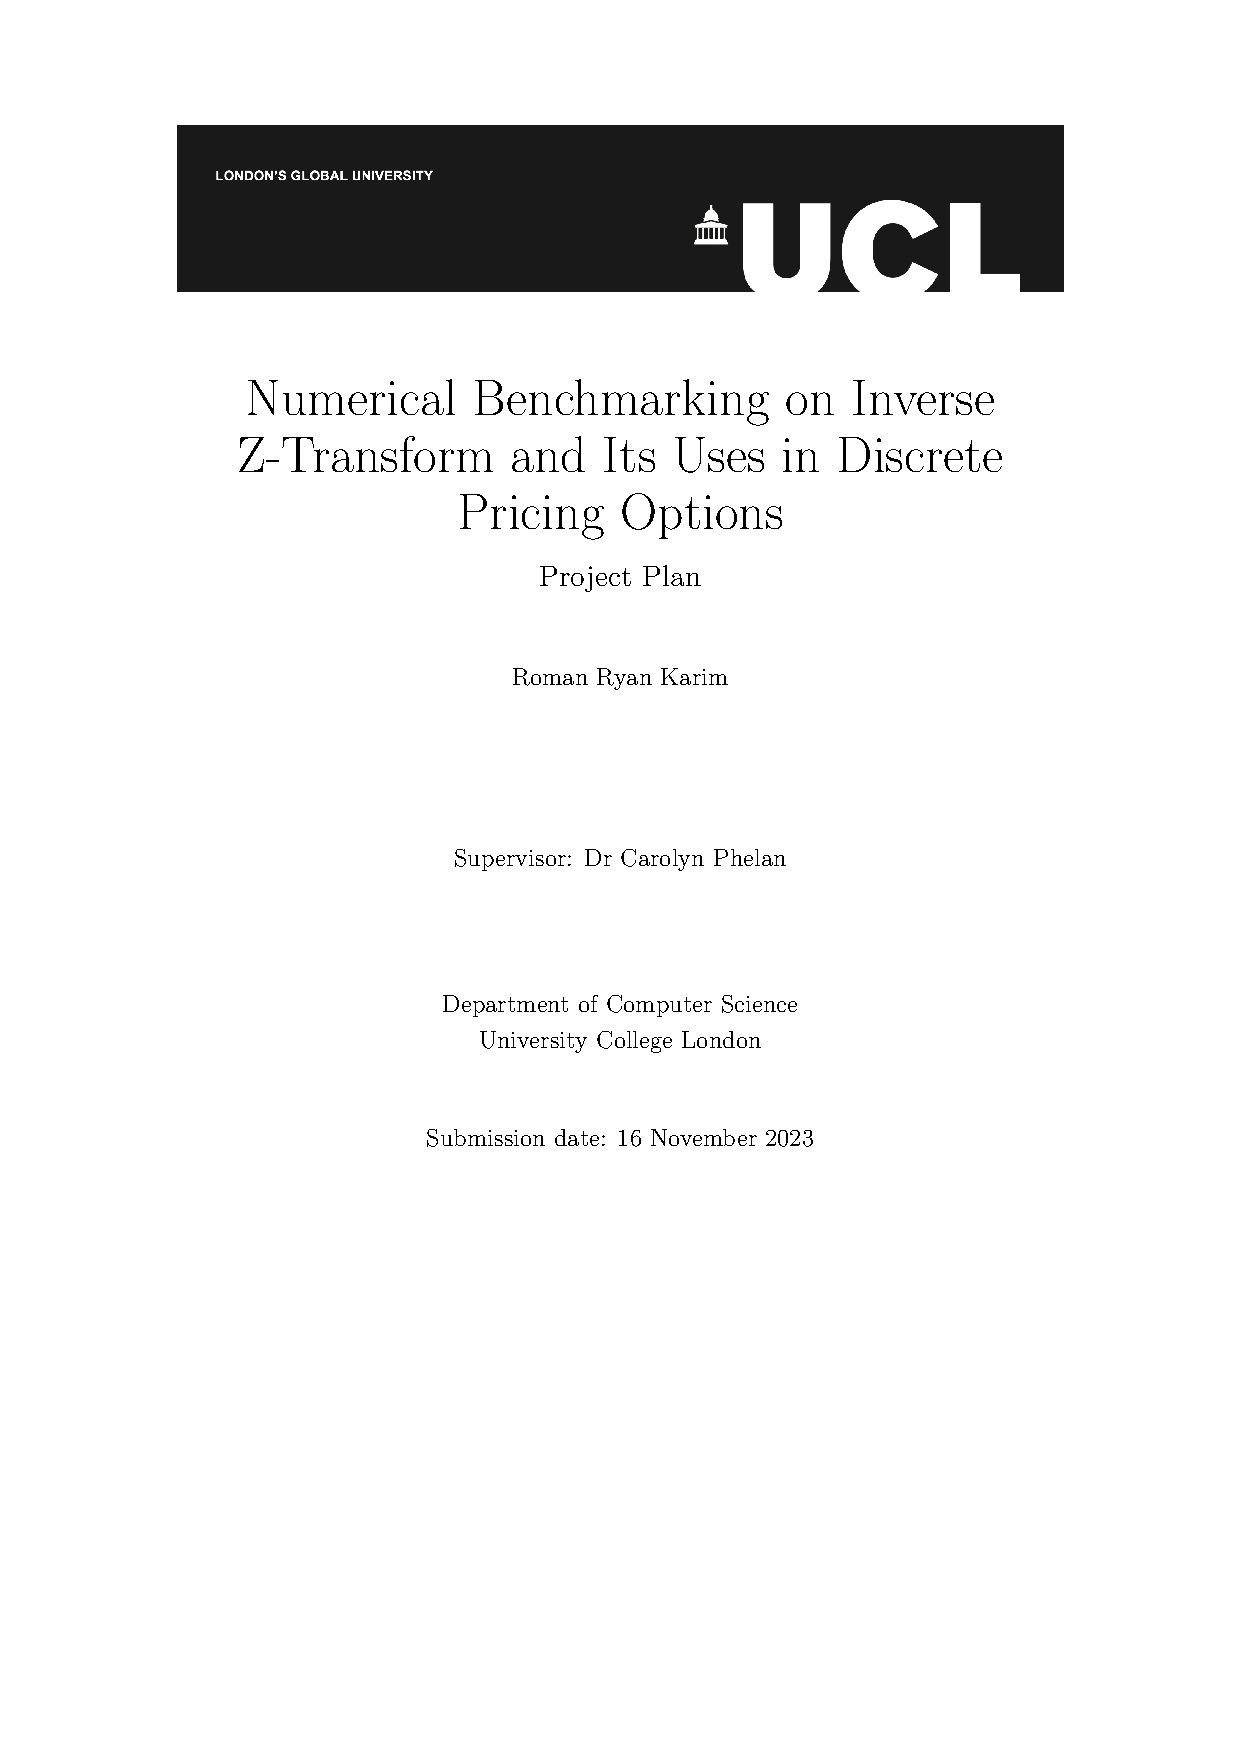
\includepdf[pages=-]{initial_project_plan.pdf}
    
\end{appendices}

\end{document}